\documentclass[12pt]{article}
\usepackage[normalem]{ulem}
\usepackage{amsmath}
\usepackage{fancyhdr, lastpage}
\usepackage{array}
\usepackage{graphicx}
\usepackage{multirow}
\usepackage{url}
\usepackage{chngpage}
\usepackage{listings}
\usepackage[pdfborder=0]{hyperref}
\usepackage[
top    = 2.75cm,
bottom = 2.50cm,
left   = 3.00cm,
right  = 3.00cm]{geometry}
\renewcommand{\refname}{}
\setcounter{secnumdepth}{5}
\setcounter{tocdepth}{6}
\lhead{Student Number: 120056321}
\rhead{Ryan Gouldsmith}
\lfoot{Aberystwyth University / Computer Science}
\cfoot{}
\rfoot{\thepage{}  of  \pageref{LastPage}}
\pagestyle{fancy}
\begin{document}
\thispagestyle{plain}
\begin{flushleft}
\rule[0.2cm]{13.8cm}{0.02cm}
\end{flushleft}
{\fontsize{15}{15}\selectfont \textbf {\centerline{CS27020: Ski Lifts and Pistes}}}
\begin{flushleft}
\rule[0.2cm]{13.8cm}{0.02cm}
\end{flushleft}
\vspace{5.2cm}
\hfill\begin{minipage}{\dimexpr\textwidth-3.0cm}
\begin{tabular}{l l}
\multirow{1}{*}{\textit{Author: }}& Ryan Gouldsmith (ryg1) \\
\\ \multirow{1}{*}{\textit{Date} } & \today \\
\\ \multirow{1}{*}{\textit{Student Number:}}& 120056321 \\ 
\end{tabular}
\end{minipage}
\newpage
\begin{center}
    \Large{
    \textbf{Abstract}}
\end{center}
In this assignment for CS27020, I have implemented a relational database from a scenario and data received in a specification. Inside is the Un-Normalized form, followed by the Normalization of the database. Finally, I have put the information into a PostgeSQL database, with accompanying screen shots of both the creation of the tables and the SQL queries which I executed. \\\\
\textbf{Notation}
For this assigment there are some notations which I need to use, to make it easier to understand some are:
\begin{enumerate}
	\item Primary Key : \uline{Primary Key}
	\item Foreign Key: Foreign Key*
	\item Functional Dependency: A $\rightarrow$ B
	\item Composite Primary and Foreign Key: (\uline{Comp1}*, \uline{Comp2}*)
\end{enumerate}
\newpage
\tableofcontents{}
\newpage
\section{Un-Normalized Structures}
\textbf{Note:} I will be normalizing the structures separately and bringing the resultant design together in the Optimise the whole set of Normalised Relations section, as shown in prior examples of the Llandwp College normalization [1].
\subsection{Piste}
\vspace{0.4cm}
This is the un-normalizard form for the Piste structure. The following design has been made upon the piste sample table.
\newline \newline
{\setlength{\extrarowheight}{10pt}
\begin{tabular}{|l|}
\hline
	\uline{PisteID}\\
	PisteName \\
	Grade  \\
	Length\\
	Fall\\
	Liftname ) Repeat\\
	isopen\\
\hline
\end{tabular}} ~\\ \\
\textbf{Note:}  LiftName repeat in this table, as a result, this will need to be moved to it's own relation in 1NF.~\\
\par{\textbf{Piste}(\uline{PisteID}, PisteName, Grade, Length, Fall, Liftname, isopen)}
\subsubsection{Functional Dependencies Piste}
Below is the Functional dependencies I feel that are required as part of my Piste design. Additionally, there are additional assumptions made on behalf of my resulting decision, these shall be fully explained.\\\\
\-\hspace{1.8cm}
\textbf{PisteID} $\rightarrow$ PisteName, Grade, Length, LiftName, Fall, isopen~\\
\noindent Above is a functional dependency for the ID key that I decided to add as a design decision, which is explained below. However, since the ID key uniquely identifies any given Piste then I feel that the PisteID has a functional dependency on all the attributes in the Piste relation, and not just the PisteName. Therefore for every instance of the same PisteID then there should be the same corresponding data.
~\\\\
\-\hspace{1.8cm}
\textbf{PisteName} $\rightarrow$ Grade, Length, Fall, isopen~\\
From the original set of Data items this is the functional dependency. This functional dependency is still valid, as all the attributes(Grade, Length, Fall, isopen) are all still dependent on the Name. Thus, this functional dependency is still valid.
\paragraph{Justification of Design and Keys}\mbox{}\\
I feel that PisteName would be a good candidate key for the data we have received because from the sample data the values for PisteName never repeat in the table. I feel that because of this, I think this is a unique key and should be considered to be a candidate key. However, I added an extra ID key. I added this key on the caution in case there happens to be two pistes with the same name but different data, this would break the integrity of the database. Finally, I feel that having the ID as an Int means that it will have quicker computational comparing times, and this making searching quicker. Additionally, I feel that the PisteName may change, and you shouldn't really be editing the primary key. However, this means that I will have to put unique constraints onto the candidate key PisteName. As a result, I have added PisteID as a surrogate key, and not used a natural key in this instance therefore PisteID is my primary key.
\subsection{Lift}
\vspace{0.4cm}
\par{This is the un-normalizard form for the Lift structure}
\newline \newline
{\setlength{\extrarowheight}{10pt}
\begin{tabular}{|p{2.5cm}|}
\hline
	\uline{LiftID}\\
	LiftName\\
	Type \\
	Summit\\
	Rise\\
	Length \\
	Operating\\
\hline
\end{tabular}} ~\\\\
\par{\textbf{Lift}(\uline{LiftID}, LiftName, Type, Summit, Rise, Length, Operating)

\subsubsection{Functional Dependencies Lift}

\par{ Below is the Functional dependencies I feel that are required as part of my Lift design. Additionally, there are additional assumptions made on behalf of my resulting decision, these shall be fully explained as I write them.\\\\}
\-\hspace{1.8cm}
\textbf{LiftID} $\rightarrow$ LiftName, Type, Operating, Rise, Length, Summit~\\
The functional dependency above indicates the new dependency which includes a LiftID - this means that all the attributes in the relation are fully dependent on the LiftID. By having this, it normally makes normalization easier to follow. As well as every instance of the same LiftID will produce the same data results.~\\\\
\-\hspace{1.8cm}
{\textbf{LiftName} $\rightarrow$ Type, Operating, Rise, Length, Summit}~\\
Above is the functional dependency for the Liftname attribute prior to me adding the LiftID key into the relation. As you can see all the attributes in the relation are dependent on the whole LiftName. This makes LiftName a good option for a candidate key.
\paragraph{Justification of Design and Keys}\mbox{}\\
For the Lift relation I feel that there are two candidate keys LiftID and LiftName, I think that both of these attributes are good candidates for the primary key. However, I feel that the LiftName may change over time. Additionally by having a String as a primary key this could mean that there's slow computational time. Therefore, I have opted for a better alternative and gone for LiftID as my primary key, this is an int and will uniquely identify the correct piste and lift, and as a result I added a surrogate key (LiftID) instead of using a natural key.
\section{Normalization}
\subsection{First Normal Form}
\textbf{Definition:} For a relation to be in first normal form 	we need to remove any duplicate attributes within a tuple by putting them into their own separate relation with the primary key of the other relation.	
\subsubsection{Piste}
As I declared in my initial design of the un-normalized structures, the attribute LiftName repeated. As a result, following the principles of first normal form we shall move LiftName out to it's own relation with the primary key of the Piste table (PisteID) linking the two tables. Thus below, is the first normal form for the Piste Example:~\\\\
\-\hspace{1.8cm}\textbf{Piste}(\uline{PisteID} PisteName, grade, length, fall, isopen)~\\
\-\hspace{1.8cm}\textbf{PisteLift}(\uline{PisteID}*,LiftName)~\\\\
As a result of the normalization we will have the following functional dependencies:
\-\hspace{1.8cm}\textbf{PisteID} $\rightarrow$ PisteName, Grade, Length, all, isopen~\\
\-\hspace{1.8cm}\textbf{PisteID} $\rightarrow$ LiftName ~\\
\-\hspace{1.8cm}\textbf{PisteName} $\rightarrow$ Grade, Length, Fall, isopen~\\
So all the information now in Piste is dependent on the PisteID. There is a dependency now on PisteID and LiftName, but this might be merged with another key in the resulting design, as LiftName isn't a key in the Lift relations and thus, we have no way of linking the two relations together.
\subsubsection{Lift}
The Lift relation are already in 1NF because there is no repeating attributes in the lift relation, thus there is no need in moving it a new relationand as a result it is already in 1NF Therefore the 1st Normal Form for Lift is: ~\\\\
\-\hspace{1.8cm}\textbf{Lift}(\uline{LiftID}, LiftName, Type, Summit, Rise, Length, Operating)~\\\\
As a result of the normalization the functional dependency is:~\\
\-\hspace{1.8cm}\textbf{LiftID} $\rightarrow$ LiftName, Type, Operating, Rise, Length, Summit~\\
\-\hspace{1.8cm}{\textbf{LiftName} $\rightarrow$ Type, Operating, Rise, Length, Summit}~\\
As a result of the first normal form the functional dependency has resulted in the same as when we declared them for the un-normalized form - this makes sense as we haven't adjusted the relation - so the dependency will not have changed. 
\subsection{Second Normal Form}
\textbf{Definition:} For a relation to be in 2NF then the relations must be in 1NF and all attributes are dependent on the whole key.
\subsubsection{Piste}
From the 1st Normalized form we can conclude that all the attributes in Piste is dependent on PisteID, and that in the PisteLift, the LiftName is dependent on the PisteID. So for our relations to be moved into 2NF then  we need to make sure that all the information is dependent on the Primary Keys. So using the functional dependency below:~\\\\
\-\hspace{1.8cm}\textbf{PisteID} $\rightarrow$ PisteName, Grade, Length, all, isopen~\\
\-\hspace{1.8cm}\textbf{PisteID} $\rightarrow$ LiftName ~\\
\-\hspace{1.8cm}\textbf{PisteName} $\rightarrow$ Grade, Length, Fall, isopen~\\\\
We can conclude that from the functional dependencies that all the attributes are dependent on the PisteID for the Piste table and that Liftname is dependent on the PisteID in the PisteLift table. This means that the structures above are aready in 2NF leaving the 2NF design as:~\\\\
\-\hspace{1.8cm}\textbf{Piste}(\uline{PisteID} PisteName, grade, length, fall, isopen)~\\
\-\hspace{1.8cm}\textbf{PisteLift}(\uline{PisteID}*,LiftName)
\subsubsection{Lift}
From the 1st normalized form then we conclude that all the attributes in Lift are dependent on the LiftID. By this logic and the functional dependency below we can conclude the 2NF for Lift.~\\\\
\-\hspace{1.8cm}\textbf{LiftID} $\rightarrow$ LiftName, Type, Operating, Rise, Length, Summit~\\
\-\hspace{1.8cm}{\textbf{LiftName} $\rightarrow$ Type, Operating, Rise, Length, Summit}~\\
Using the above functional dependency we can clearly see that all the attributes in the Lift is dependent on the primary key And thus the relation is already in the 2nd Normal Form for Lift. Below is the resultant 2NF:~\\
\-\hspace{1.8cm}\textbf{Lift}(\uline{LiftID}, LiftName, Type, Summit, Rise, Length, Operating)
\subsection{Third Normal Form}
\textbf{Definition:} For a relation to be in 3NF all the attributes must be in 2NF and there must be no transitive dependencies.
\subsubsection{Piste}
The Piste relations so far are in 2NF. Therefore using the functional dependencies I can check to see if there's a third normal form. Below are the functional dependencies for Piste:~\\\\
\-\hspace{1.8cm}\textbf{PisteID} $\rightarrow$ PisteName, Grade, Length, Lifts, Fall, isopen~\\
\-\hspace{1.8cm}\textbf{PisteName} $\rightarrow$ Grade, Length, Fall, isopen~\\
\-\hspace{1.8cm}\textbf{PisteID}$\rightarrow$ LiftName~\\
Above are the dependencies on Piste. Although there seems that there might be a transitive dependency on PisteID and PisteName, there infact isn't. This is because, PisteName is a subset of PisteID - therefore, it's not a transitive dependency. As a result, there are infact no transitive dependencies in the relations that I have designed, and PisteLift can't have any transitive dependencies as it only has two attributes. As a result the Piste is already in 3NF. And as a result the third normal form for Piste is below:~\\\\
\-\hspace{1.8cm}\textbf{Piste}(\uline{PisteID} PisteName, grade, length, fall, isopen)~\\
\-\hspace{1.8cm}\textbf{PisteLift}(\uline{PisteID}*,LiftName)
\subsubsection{Lift}
The Lift relation is already in 2NF, so to ensure that it's in 3NF I need to make sure that the Lift relation does not contain any transitive dependences. Below are the functional dependencies: ~\\\\
\-\hspace{1.8cm}\textbf{LiftID} $\rightarrow$ LiftName, Type, Operating, Rise, Length, Summit~\\
\-\hspace{1.8cm}\textbf{LiftName} $\rightarrow$ Type, Operating, Rise, Length, Summit}~\\
Here, like the Piste example, there may seem a transitive dependency between LiftID, LiftName and all the attributes to do with a lift. However, because that LiftName is a subset of LiftID, much like Piste then it can't be a transitive dependency, and all the data is still dependent on the Primary Key LiftID. Thus, this shows that there is no transitive dependency on Lift, which means that the Lift is already in 3NF; below is my final 3NF for the Lift relation:~\\\\
\-\hspace{1.8cm}\textbf{Lift}(\uline{LiftID}, LiftName, Type, Summit, Rise, Length, Operating)
\subsection{Optimising The Whole Set Of Normalized relations}
So, I have normalized all my structures separately and now I wish to bring them together to show how they all link together. Inside this section there might be some slight design changes, but these shall be justified. From the normalization process of both, Piste and Lift, we have the following relations which total 3 relations:~\\\\
\-\hspace{1.8cm}\textbf{Lift}(\uline{LiftID}, LiftName, Type, Summit, Rise, Length, Operating)~\\
\-\hspace{1.8cm}\textbf{Piste}(\uline{PisteID} PisteName, grade, length, fall, isopen)~\\
\-\hspace{1.8cm}\textbf{PisteLift}(\uline{PisteID}*,LiftName)~\\\\
Now, using decisions based on the requirements specification and experience of the given task, I will now bring them together to form my final set of relations. The LiftName in the PisteLift relation will be replaced with the Primary Key in the Lift relation LiftID. This needed to be implemented because without the LiftID key been added the PisteLift relation then there would be no way of keeping track of which Lift is associated to which ID. So replacing the LiftName attribute to LiftID hasn't changed anything, it has only changed the way we will refer to the lifts; since LiftName is dependent on LiftID, then we know this is valid. As a result, we have taken our many-to-many relationship and normalized it. And as a result come out with a set of relations below.~\\\\
\-\hspace{1.8cm}\textbf{Piste}(\uline{PisteID} PisteName, grade, length, fall, isopen)~\\
\-\hspace{1.8cm}\textbf{Lift}(\uline{LiftID}, LiftName, Type, Summit, Rise, Length, Operating)~\\
\-\hspace{1.8cm}\textbf{PisteLift}(\uline{PisteID}*,\uline{LiftID}*)
\newpage
\section{PostgreSQL implementation}
\subsection{Create Tables}

\lstinputlisting[frame=single, language=sql, breaklines=true]{create_tables.sql}
\subsubsection{Justification Of Design}
Above is the script in which I used to generate the relations for my Database. I will give a justification on the datatypes I have used, and why I feel they're best suited to my design.
~\\\\
First off, I have 3 statements at the top of the script where I drop any tables if they've already been implemented. I feel that this would be good in the create\_tables.sql script as if you're making changes to the tables, then you will want to delete the other tables too. 

In the Piste script I used Serial as a datatype for the primary key. After some research I found that Serial has a minimum value of 1 and a maximum value of 2147483647 [2] So I thought this would be sensible for the primary key and I wouldn't have to include any extra checks to ensure that the data is valid, along with this the Serial key is auto incrementing. Secondly, I used the Datatype VarChar to size 100 on PisteName as I felt that some of the Piste names are very long in the sample data, so in theory they could be even longer - thus this covers it. Additionally on this datatype I have added two constraints; as  PisteName is a candidate key in my design I had to ensure that all the values entered into this field were unique, this has been covered with the key word UNIQUE - thus meaning each value in the PisteName attribute has to be different: Additionally, I have used a Not Null statement so that the values have to contain some data - this is also follows on from my functional dependency statement.
Grade is given type gradevalue which is an enumerated type - this provides data integrity as it means that there can only be a set values to choose from. I had to use real on length as it was the lowest data type which allowed the storage of decimal values. I enforced a check on this datatype so that the length was always \textgreater 0, this means that there can not be any negative lengths and thus making the data more integral.
Fall is type smallint: I chose this because it was the most sensible data type the fall as it allowed the size of the fall to be enough, but not wasting any unwanted size on an int. Additionally, I added a check constraint to make sure that that the fall, too, couldn't be in negative numbers.
Finally, I used an enum for isopen called openvalue which stores a yes or no result. I appreciate I could have used a boolean type but I decided to choose readability over performance as t and f was difficult to read.
~\\\\
In the second relation, Lift, again used Serial for my autoincremented Primary ID key, this is the same as Piste, this doesn't need to have NOT NULL as it will always increment and therefore be NOT NULL. I also put a constraint on liftname to make it UNIQUE - thus meaning that any liftname must be Unique, this follows on from my normalization process where I identified liftname as a candidate key. I also gave lift type an Enumerated type of liftype, as there was only a selection of lifttypes that I thought this would be valid as there is only a small selection of lifttypes available, so to enforce data integrity I added the enumerated type, see below for my justification on enums. Again I used small int for summit, rise and length as this was the smallest datatype which fitted the sample data thus using less space, and as stated in Piste, I feel that using real world knowledge that these values will not go over the maximum value for smallint. Finally again, I used an enumerated type for open value, which is the same as Piste, and again, I used this over readability instead of using TRUE or FALSE. Finally I gave summit, rise and length a check constraint to ensure that all the values are \textgreater 0. As a result this means we can not add any negative numbers in as these values, which makes the data more reliable.
~\\\\
The PisteLift Table, is the table for linking the Many to Many relationship. So in this relation I have two ID keys, piste and lift. These are both type SERIAL since this is the type we used in the prior tables as Primary Keys, these have a foreign key reference to pisteID and liftID respectively. Finally, we have both these keys making up one composite Primary Key, as any single relation needs to have a Primary key attached to it - both of these are Unique and this is how we set up the lookup table.
~\\\\
Now I am going to justify the use of an enumerated type, seen at the top of the create tables script. I recognise that I could have used another relation and had either: Operating, lifttype or gradevalue as separate relations and linked them to the previous table via a foreign key reference. However I did not because of the following: You can easily add to the enumerated type, it makes queries easier as you don't have to reference another table, and as I will be referencing a few tables to get a desired output then this is more efficient. So, overall, I feel that an enum is an easy way to check for integrity in the database, and I felt that it would be the better solution for this design.
~\\\\
Finally, all the attributes in my create table have a NOT NULL constraint, this means that you have to add data into these attributes. I made this decision based upon my functional dependency and real knowledge example, that all the information will have to be provided to make sense. This just adds integrity to the database to make sure that all the values have to be inserted correctly.
\newpage
\subsection{Inserting Data}
\lstinputlisting[frame=single, language=sql, breaklines=true]{insertvalues.sql}

Above is a sample of the data inserted into my database. This is added for completeness, and to show my use of data for the queries.
\newpage
\subsection{Queries}
\subsubsection{Query 1}
\lstinputlisting[frame=single, language=sql, breaklines=true]{query1.sql}
\begin{figure}[htp]
\begin{adjustwidth}{-0cm}{0cm}
\centering
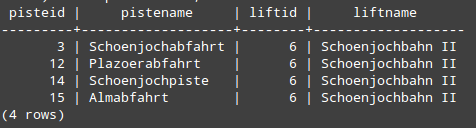
\includegraphics[scale=0.80]{Screenshots/query1upd(copy).png}
\caption{Result of Query 1}
\label{Query 1}
\end{adjustwidth}
\end{figure}
For this query I had to search for the Pistes served by a given Lift. Now, here, first of I decided that it would be more appropriate to return the pistename and liftname and no other data. I interpreted the query as returning the pistenames from a given lift; as a result I just returned the name as I felt I didn't have to return all the data about the piste. However, since I used ID for the search you did have to know the ID number of the lift in order to do this. Again, the requirements stated that we didn't have to search by name, however, if you were to search by name you would replace the where clause with: \textbf{WHERE l.liftname='Schoenjochbahn II';} and this would produce the same result. I decided that it would be easier to search by the key ID. I decided to use an INNER JOIN on the tables over nested select statements as it was easier to read than nested select statements, as well, the INNER JOIN returns all the tuples, as long as there's a match in the attribute, thus all the other data will not be included. I decided to join the relations on the ID's as this improved the speed of the query. Finally, I used pl for the piste lift table, p for the piste table and l for lift because it meant the query wasn't as long, and it is still readable. (this is a common theme through all the queries)
\subsubsection{Query 2}
\lstinputlisting[frame=single, language=sql, breaklines=true]{query2.sql}
\clearpage
\begin{figure}[htp]
\centering
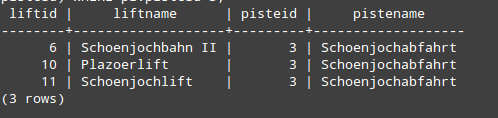
\includegraphics[scale=0.80]{Screenshots/Query2Upt(copy).png}
\caption{Result of Query 2}
\label{}
\end{figure}
For the second query I had to search for lifts that serve a given piste. Again, this is very similar to the query 1, but I selected all the information from Lift and Joined the PisteLift on the ID and Piste On the ID too, I then searched for a piste via the ID of the piste, rather than the name. Again, I thought that since the requirements of the query only stated to return the lift, I decided to only return the name of the lift, the lift ID, the piste ID and the pistename so you know which piste is available to see. Additionally, I did it this way as that was it's easier to see which lifts are served by a given piste, rather than loads of data that may not be necessary for this example. Again, like query 1, I could have changed the where clause to be slighty more readable such as: \textbf{WHERE p.pistename='Schoenjochabfahrt';} but I since the names are long and complex this could lead to error, and you would most likely have to look up the name - which whilst doing so you can get the id and thus have a quicker search. Again, I used INNER JOIN instead of nested statements so that we can quickly join tables and make searching easier. Another thing to note, I joined the Piste and Lift tables to get the names, so we can see the associated ID's, rather than just a list of ID's - this means that there's improved readability in the results. Finally, I used pl for the piste lift table, p for the piste table and l for lift because it meant the query wasn't as long, and it is still readable.
\subsubsection{Query 3}
\lstinputlisting[frame=single, language=sql, breaklines=true]{query3.sql}
\clearpage
\begin{figure}[htp]
\centering
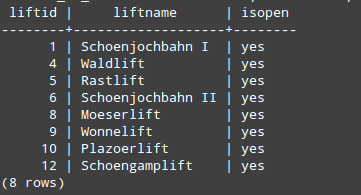
\includegraphics[scale=0.60]{Screenshots/query3UPD(copy).png}
\caption{Result of Query 3}
\label{}
\end{figure}
This third query was simple enough. I used a select statement which returned the liftid, liftname and isisopen value from the lift table where isopen is equal to yes. I decided to just query the table since there was no need for added complications with this query. Additionally, I feel this is where the table for enum yes and no are advantageous - as it makes the table easier to read, rather than t or f.Finally, I used pl for the piste lift table, p for the piste table and l for lift because it meant the query wasn't as long, and it is still readable.
\subsubsection{Query 4}
\lstinputlisting[frame=single, language=sql, breaklines=true]{query4.sql}\begin{figure}[htp]
\centering
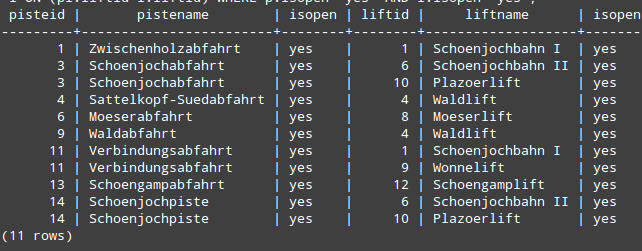
\includegraphics[scale=0.55]{Screenshots/query4upd.png}
\caption{Result of Query 4}
\label{}
\end{figure}
This 4th query was the hardest query of them all. It returns the pistes that are open, as the lifts that are open and that provide service to the pistes. So for this, I thought the table result would be rather large, so again I narrowed it down to just the pisteid, pistename, isopen, liftid, liftname and isopen on the lift - as a result the table is much easier to read. Again, I used inner joins but this time I selected all the values from PisteLift as it concerned both relations I thought that this might have been the better solution. As well as this, I used the WHERE piste is open AND lift isopen. As we were looking for the results of both of them I thought an AND would be more appropriate. Again I used the INNER JOIN over nested statements especially as the statements got longer it made it easier to read. Finally, one other decision I made was to give piste, lift and pistelift a shortened name, although this may confuse things slightly, if read properly it makes sense and makes the query shorter and less verbose.
\subsubsection{All Piste Data}
\lstinputlisting[frame=single, language=sql, breaklines=true]{query5.sql}
\begin{figure}[htp]
\centering
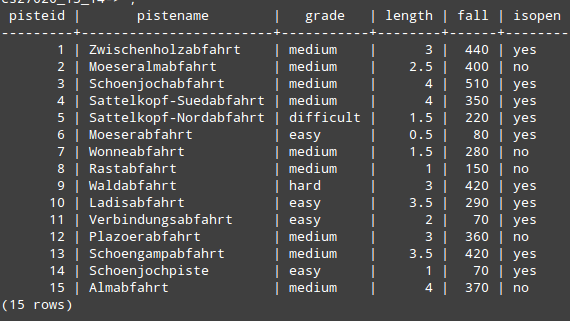
\includegraphics[scale=0.545]{Screenshots/AllPiste.png}
\caption{Result of Query 5}
\label{Query of select all the Data from the Piste table}
\end{figure}
This query is only included so you can see that I can query all the data inside the piste table, as I didn't output the whole piste table in the queries that were requested in the assignment because I felt that all the data didn't need to be shown. So now you can see all the information which is related to a given piste and that there are no duplicated data items.
\subsubsection{All Lift Data}
\lstinputlisting[frame=single, language=sql, breaklines=true]{query6.sql}
\begin{figure}[htp]
\centering
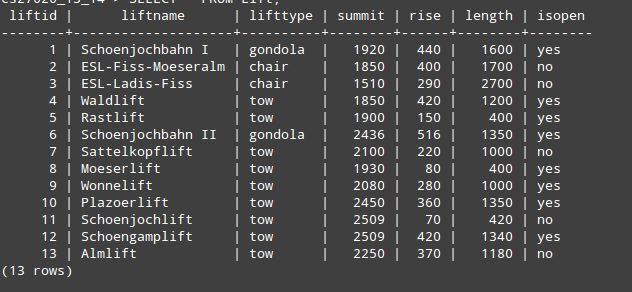
\includegraphics[scale=0.5]{Screenshots/AllLift.png}
\caption{Query of Selecting all the Data from the Lift table}
\label{}
\end{figure}
This query is only included so you can see that I can query all the data inside the table, as I didn't output the whole table in the queries that were requested in the assignment because I felt that all the data didn't need to be shown. So instead I just wrote an extra script to show each lift with all the associated values with it.\subsubsection{All PisteLift Data}
\lstinputlisting[frame=single, language=SQL, breaklines=true]{query7.sql}
\begin{figure}[htp]
\centering
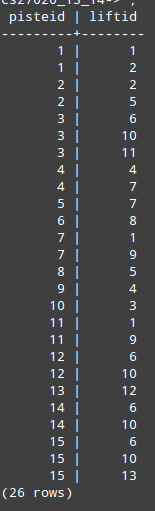
\includegraphics[scale=0.45]{Screenshots/PisteLift.png}
\caption{Query of Selecting all the data from the joining table}
\label{}
\end{figure}
I decided to add this into the selection of screen shots such that I can show that I can select all the data associated with the the joining tables, as in the queries provided I have narrowed down the selection. Also, this shows that I can use Select all on a table and it will show the sample data I have got.
\newpage
\section {Conclusion}
Overall, I feel that the assignment went well. I thought that there were sections which were unclear, and I got this clarified off of Edel. Having used databases before, but not normalizing them since college I found this tricky especially with information on the Internet telling you differently. However, I used the worked examples that were on the department website and in the end everything made sense. I had a bit of an issue with functional dependencies especially with the transitive ones, but this was sorted relatively quickly. Although parts of the exercise seemed relatively simple, I see that the design is up to you as along you justify it. Additionally, working out the functional dependency really did help with working out the normalization process.

I found writing the scripts simple, as I have written SQL scripts before. What was interesting was some of the PostgreSQL syntax used was slightly different than MySQL and caught me out occasionally. However, writing the syntax for the SQL statements wasn't too difficult as I have used Joins before and therefore knew that they worked for situation, so it was mainly remembering the syntax.

So in general I learnt a lot about the process of database design and normalization. With a mixture of looking up pieces of information because my knowledge was hazy to what was the smallest data type in PostgreSQL - I feel that I have learnt a lot from the assignment.

\section {References} 
\begin{thebibliography}{}
\bibitem{College}
Edel Mary Sherratt. Bottom up Analysis.\url{http://www.aber.ac.uk/~dcswww/Dept/Teaching/CourseNotes/current/CS27020/Lectures/LlandwpWorkedExample.pdf} [February 2014]
\bibitem{hjdfs}
PostgreSQL. Data Types. \url{http://www.postgresql.org/docs/9.3/interactive/datatype.html}[February 2014]
\bibitem{Enums}
O'Reilly. Enumerated Types. \url{http://www.oreillynet.com/pub/a/databases/2006/01/06/enumerated-fields-in-postgresql.html} [February 2014]
\end{thebibliography}
\end{document}